\chapter{HADES Event Display}\label{Chapter_eventdisplay}


\begin{figure}[\htb]
\begin{center}
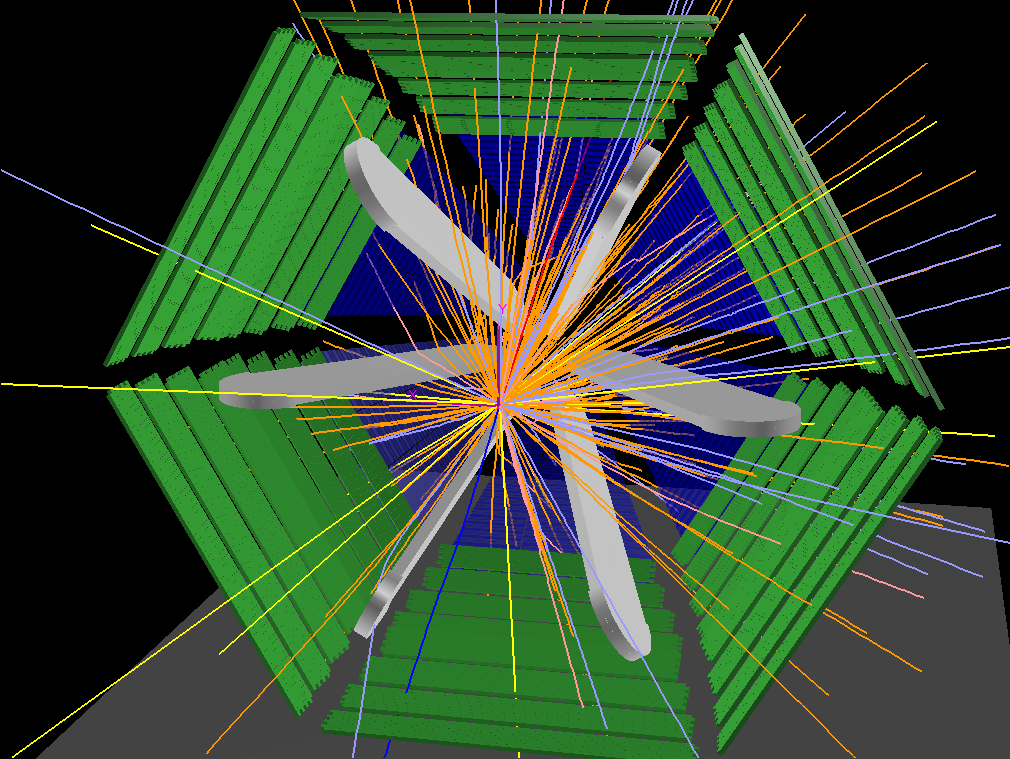
\includegraphics[width=0.8\linewidth,clip=true]{pics/eventdisplay/hades_au17au_sim_geant_iso_dark.png}
\caption[Eventdisplay for HGeant tracks]{Eventdisplay for HGeant tracks.} \label{eventdisplay_geant}
\end{center}
\end{figure}

\begin{figure}[\htb]
\begin{center}
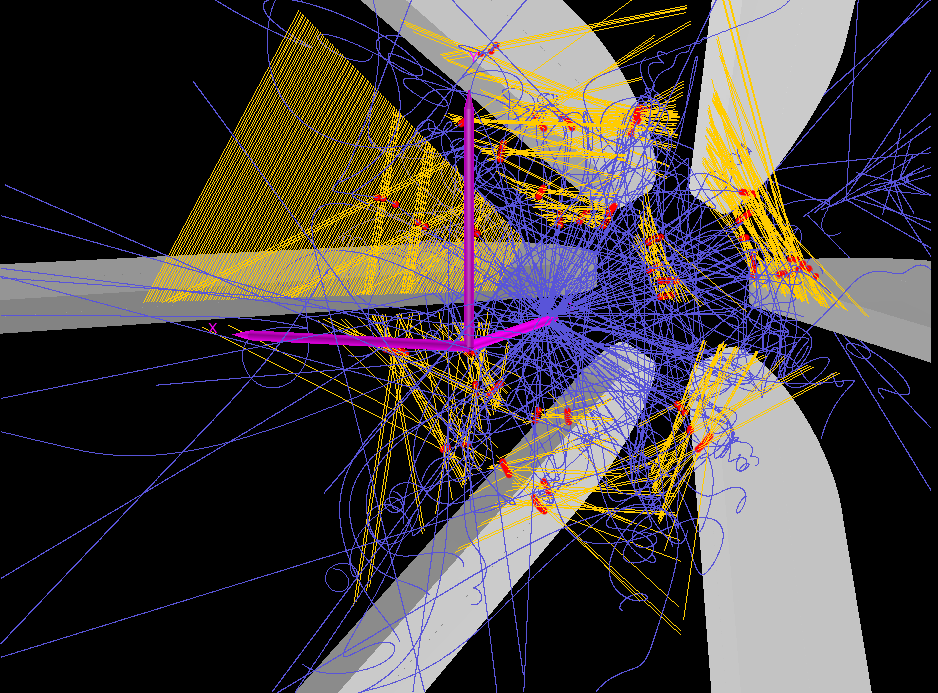
\includegraphics[width=0.8\linewidth,clip=true]{pics/eventdisplay/evt51_deltaelectrons_wires.png}
\caption[Eventdisplay for HGeant tracks]{Eventdisplay for HGeant tracks. Delta electron close
to the magnet coils.} \label{eventdisplay_deltas_geant}
\end{center}
\end{figure}



The Hades evcent 3D display is build on pure ROOT technology.
It makes use out of the ROOT build in \verb+TEve+ display and 
\verb+TGeoManager+.
It uses openGL and therefore can be used on local and remote 
(via X11) place but not via VNC (since VNC does not support openGL).

The HADES eventdisplay is provided by macros located in
the HYDRA2 module eventdisplay and the compiled library
\verb+libEventDisplay.so+ created during the standard 
make of HYDRA2.

The display uses \verb+TGeoManager+ to display the HADES detector
geometry. A ROOT file containing +TGeoManager+ can be created
by a macro. As input for the display the ROOT file is used.
The library provides objects to display hits of the different
detectors and and automtic filling of this objects from
the standard analysis objects.


\section{HOWTO setup}

To run the prepared example for central Au+Au@1.5AGeV collisions: 
\begin{lstlisting} [language=bash]

 Copy all macros HYDRA/eventdisplay/*.C 
 to your local dir. You may need
 to edit them according to your needs.

 To start in ROOT session: .x eventDisplay.C+
\end{lstlisting}

A short verview over the functionanlity of the macros and
if the user need to edit them is given below:

\begin{lstlisting}
  eventDisplay.C  : USER ACTION : setup the TGeomManager root file
  loadHadesGeom.C : NO USER ACTION required here.
  make_GUI.C      : NO USER ACTION required here.

  createHades.C   : USER ACTION required here.
                    creates HADES including detectors,
                    parameter and data sources. Setup and
                    taskslists can be changed here.
                    Basically a DST macro. This example
                    is done for Au+Au@1.5AGev simulation

  nextEvent.C     : USER ACTION required here.
                    loads one HADES event into memory. Copy
                    of hits and tracks to Eve objects is
                    done here. The user can select / group
                    and change property of the displayed
                    objects. The parts where the user should
                    edit the macro are markerd
                    "######## USER ACTION #####"
\end{lstlisting}


\section{The macros}

This section decribes the functionality of the different
macros and how the are linked together in more depths.


\verb+loadHadesGeom.C+
Reads HADES geometry from root file containing \verb+TGeoManager+.
All volumes are set invisible by default and only some
selected volumes are set visible again with the desired
color and transparency. If the \verb+TEveManager+ does not
exist it will be created. The Geometry will be added
to the global scene (persistent). The pointer to the used
\verb+TGeoVolumes+ and \verb+TGeoNodes+ are stored in 
\verb+HEDColorDef+. This
object is used by the GUI for changing the properties later.
Compiled on load time. Coordinate transformations for the
RICH pad plane and mirror are stored too.

\verb+make_GUI.C+
Creates the GUI for Display setup in \verb+TEve+. Connect
"next Event" button to 
\newline
\verb+HEDEvtNavHandler+ defined in
\verb+nextEvent.C+. Compiled on load time.

\verb+nextEvent.C+
loads a new event into memory.
It performs a call to Hades event loop. After
running the event loop the full event is available
in memory. The different detector hits can be selected
by the user, tranformed and added to the event scene of
\verb+TEve+. All objects of the previous event scene will be
destroyed.
The class \verb+HEDEvtNavHandler+ is defined here. It
is event handler to connected to the GUI.
This Class provides the \verb+selectEvent()+ function connected
to the "next Event" button. The function then calls
\verb+nextEventLoop()+ or \verb+nextEvent()+ depending if 
the the loop box is checked.
\verb+HEDEvtNavHandler+ holds the user defined 
\verb+TEveElementLists+ which are inserted in the Event 
Scene of \verb+TEveManager+. The user has to clean and 
fill this lists inside \verb+nextEvent()+.
The lists appear in "Eve" tab of the GUI in the browser
"Scenes/Event scene". The parts where the user should
edit the macro are markerd \verb+"######## USER ACTION #####"+
Compiled on load time.

\section{Available graphic objects}

The available graphic objects are defined
\verb+libEventDisplay.so+, (\verb+hedhitobjects.h+,
\newline
\verb+hedhelpers.h+)

The Eventdisplay uses LAB coordinates with x,y.z units 
in mm. Hence all hits objects from the analysis have to be
transformed to LAB and cm (TEve units). Functions used 
for coodinate transformations are located in \verb+HEDTransform+. 
\verb+HEDMdcWireManager+ will do the count statistics for 
the MDC wires. \verb+HEDGroup+ and \verb+HEDGroup2D+ 
provide some help to group
\verb+TEveElementLists+ in 1 or 2 dim arrays. This is useful
to group graphic object like sector or sector/module.
expample:
\begin{lstlisting}
  HEDGroup* sectors  = new HEDGroup("sectors","sectors",6,"Sector");
  // will create 1 main list containing 6 lists one for each sector.
  sectors->AddElement(Int_t sector,TEveElement* el)
  // will add an object to the list of the sector. The elements
  //can be TEveElementLists allowing to create complex structures.
\end{lstlisting}

The following graphical objects to display Detector hits
and tracks are available and work for REAL/SIM data:

\begin{lstlisting}
 HEDVertex          : public TEvePointSet (no input needed)
 HEDSegment         : public TEveLine     ==> HEDSegment(HMdcSegSim*)
 HEDMdcWire         : public TEveLine     ==> HEDMdcWire(HMdcCal1Sim*)
 HEDRichHit         : public TEveLine     ==> HEDRichHit(HRichHitSim*)
 HEDRichHitPadPlane : public TEvePointSet ==> HEDRichHitPadPlane(HRichHitSim*)
                      // RICH hit at pad plane
 HEDRichRing        : public TEvePointSet ==> HEDRichRing(HRichHitSim*)       
                      // RICH ring at pad plane
 HEDRichPadPlane    : public TEveQuadSet  ==> HEDRichPadPlane(Int_t sector)   
                      // RICH pad plane + fired pads
 HEDRichCompound    : public TEveCompound ==> HEDRichCompound(HRichHitSim*)   
                      // RICH hit at pad plane + ring + mirror hit
 HEDTofHit          : public TEvePointSet ==> HEDTofHit(HTofHitSim*)
 HEDTofCluster      : public TEvePointSet ==> HEDTofCluster(HTofClusterSim*)
 HEDRpcCluster      : public TEvePointSet ==> HEDRpcCluster(HRpcClusterSim*)
 HEDShowerHit       : public TEvePointSet ==> HEDShowerHit(HShowerHitSim*)

 HEDParticleCand : public TEveCompound ==> HEDParticleCand(HParticleCandSim*)
    consist out of all detector hits contributing to
    the candidate. The object provives functions
    to change the graphical representation/

    void SetLineColor  (Color_t val)
    void SetLineStyle  (Style_t val)
    void SetLineWidth  (Style_t val)
    void SetMarkerColor(Color_t val)
    void SetMarkerStyle(Style_t val)
    void SetMarkerSize (Size_t val)
    void SetRnrLine    (Bool_t val)  // kTRUE: line  will be shown
    void SetRnrPoints  (Bool_t val)  // kTRUE: points will be shown

 HGEANT OBJECTS
 TEveTrack* track = HEDTransform::createKineParticle(kine,simTrackList->GetPropagator());
                  : HEDField keeps the HADES filed map. The Runge Kutta propagator
                  : of Eve is used to propagate the track trough the detector.
 HEDRichGeantPadPlane : to draw GEANT hits on the RICH PADplane
 HEDRichGeantMirror   : to draw GEANT Mirror hits
\end{lstlisting}


\begin{figure}[\htb]
\begin{center}
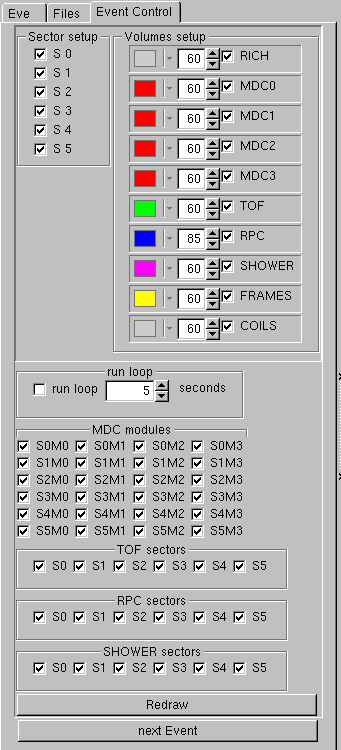
\includegraphics[width=0.4\linewidth,clip=true]{pics/eventdisplay/eventControl.png}
\caption[Eventdisplay event control]{Event control tab of the Eventdisplay. Colors , transparency 
and visability of the detectors can be set here. After the change the "Redraw" button has 
to be pressed.} \label{eventdisplay_control}
\end{center}
\end{figure}

\begin{figure}[\htb]
\begin{center}
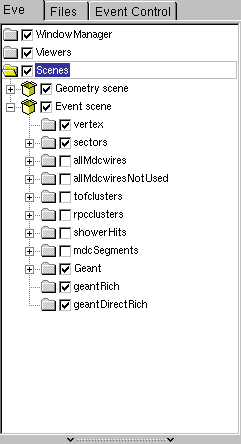
\includegraphics[width=0.4\linewidth,clip=true]{pics/eventdisplay/eveTree.png}
\caption[Eventdisplay eve tab]{Eve tab of the Eventdisplay. All graphical objects in the scene 
are eachable via this tab. The "Geometry Scene" contains the the geometrial Volumes
of the Detector. The "Event Scene" owns all objects created by the user in the "nextEvent()" 
function.} \label{eventdisplay_tree}
\end{center}
\end{figure}

\begin{figure}[\htb]
\begin{center}
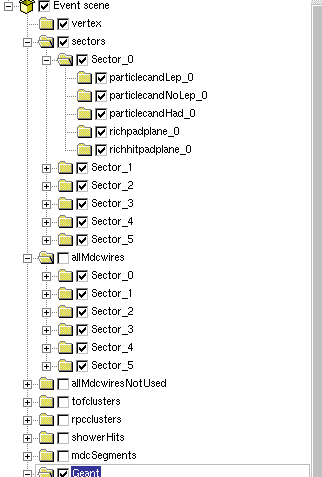
\includegraphics[width=0.4\linewidth,clip=true]{pics/eventdisplay/treeReco.png}
\caption[Eventdisplay eve tab - reco objects]{Eve tab of the Eventdisplay. 
Shown are the reconstructed objects. The objects are ordered by groups of the 
sector of the detector.} \label{eventdisplay_tree_reco}
\end{center}
\end{figure}

\begin{figure}[\htb]
\begin{center}
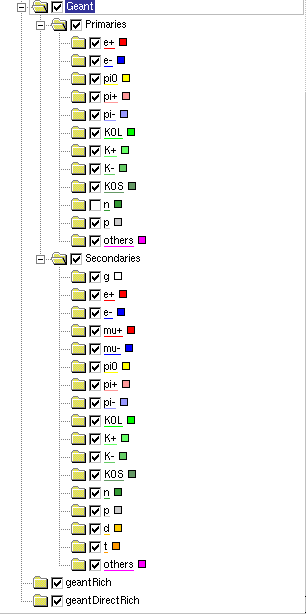
\includegraphics[width=0.4\linewidth,clip=true]{pics/eventdisplay/treeGeant.png}
\caption[Eventdisplay eve tab - HGeant objects]{Eve tab of the Eventdisplay. Shown are the HGeant 
objects. Primary and secondary particles are sorted into diffent lists. Each of the
lists keeps a list for each particle species. The particle trajectories are calulated using
the HADES magnetic field map and are propagated by a Runge-kutta algorithm through the 
detector.} \label{eventdisplay_tree_geant}
\end{center}
\end{figure}



